\section{Результаты измерений}

Длина стержня $l=0{,}9998\pm 5\cdot10^{-5}\,\text{м}\;\text{(}\varepsilon=5\cdot10^{-5}\text{)}$,
масса стержня $m_\text{с}=868{,}4\pm0{,}05\,\text{г}\;\text{(}\varepsilon=6\cdot10^{-5}\text{)}$,
масса призмы $m_\text{с}=75{,}7\pm0{,}05\,\text{г}\;\text{(}\varepsilon=7\cdot10^{-4}\text{)}$,
масса груза $m_\text{с}=376{,}2\pm0{,}05\,\text{г}\;\text{(}\varepsilon=1{,}3\cdot10^{-4}\text{)}$.

Уравновешивая стержень на призме, получим, что центр масс находится посередине.

\begin{table}[!ht]
    \centering
    \caption{Измерения на установке А}
    \begin{tabular}{|l|l|l|l|l|}
    \hline
        $a,\pm 0{,}05\,\text{см}$ & $x_c,\pm 0{,}05\,\text{см}$ & $t,\pm 0{,}005\,\text{с}$ & $T,\pm 2{,}5\cdot10^{-4}\,\text{с}$ & $g,\,\text{м}/\text{с}^2$ \\ \hline
        48 & 43.8 & 32.5 & 1.625 & 9.77 \\ \hline
        40 & 36.5 & 31.33 & 1.5665 & 9.79 \\ \hline
        37 & 33.8 & 31.2 & 1.56 & 9.65 \\ \hline
        32.5 & 29.7 & 30.76 & 1.538 & 9.7 \\ \hline
        30 & 27.7 & 30.57 & 1.5285 & 9.76 \\ \hline
        28.6 & 26.2 & 30.52 & 1.526 & 9.79 \\ \hline
        23.6 & 24.5 & 30.97 & 1.5485 & 9.7 \\ \hline
        20.3 & 18.8 & 31.57 & 1.5785 & 9.71 \\ \hline
        17.3 & 15.8 & 32.63 & 1.6315 & 9.7 \\ \hline
        14.2 & 13.1 & 34.47 & 1.7235 & 9.68 \\ \hline
        11.2 & 10.2 & 37.17 & 1.8585 & 9.78 \\ \hline
        9.7 & 8.5 & 40.1 & 2.005 & 9.39 \\ \hline
        7.2 & 6.8 & 44.32 & 2.216 & 9.88 \\ \hline
    \end{tabular}
\end{table}

Колебания при $a=30\,\text{с}$ при троекратном измерении совпали, поэтому
случайной погрешностью можно пренебречь.

По результатам таблицы $g=9{,}72\pm0{,}03\,\text{м}/\text{с}^2$.

\begin{table}[!ht]
    \centering
    \caption{Измерения на установке Б}
    \begin{tabular}{|l|l|l|}
    \hline
        $x_c,\pm 0{,}05\,\text{см}$ & $t,\pm 0{,}005\,\text{с}$ & $T,\pm 2{,}5\cdot 10^{-4}\,\text{с}$ \\ \hline
        40.7 & 32.62 & 1.631 \\ \hline
        40.1 & 32.29 & 1.6145 \\ \hline
        39.4 & 31.93 & 1.5965 \\ \hline
        38.5 & 31.57 & 1.5785 \\ \hline
        37.9 & 31.22 & 1.5161 \\ \hline
        37.2 & 30.92 & 1.546 \\ \hline
        36.1 & 30.49 & 1.5245 \\ \hline
        35.8 & 30.32 & 1.516 \\ \hline
        34.7 & 30.03 & 1.5015 \\ \hline
    \end{tabular}
\end{table}

\begin{figure}
    \centering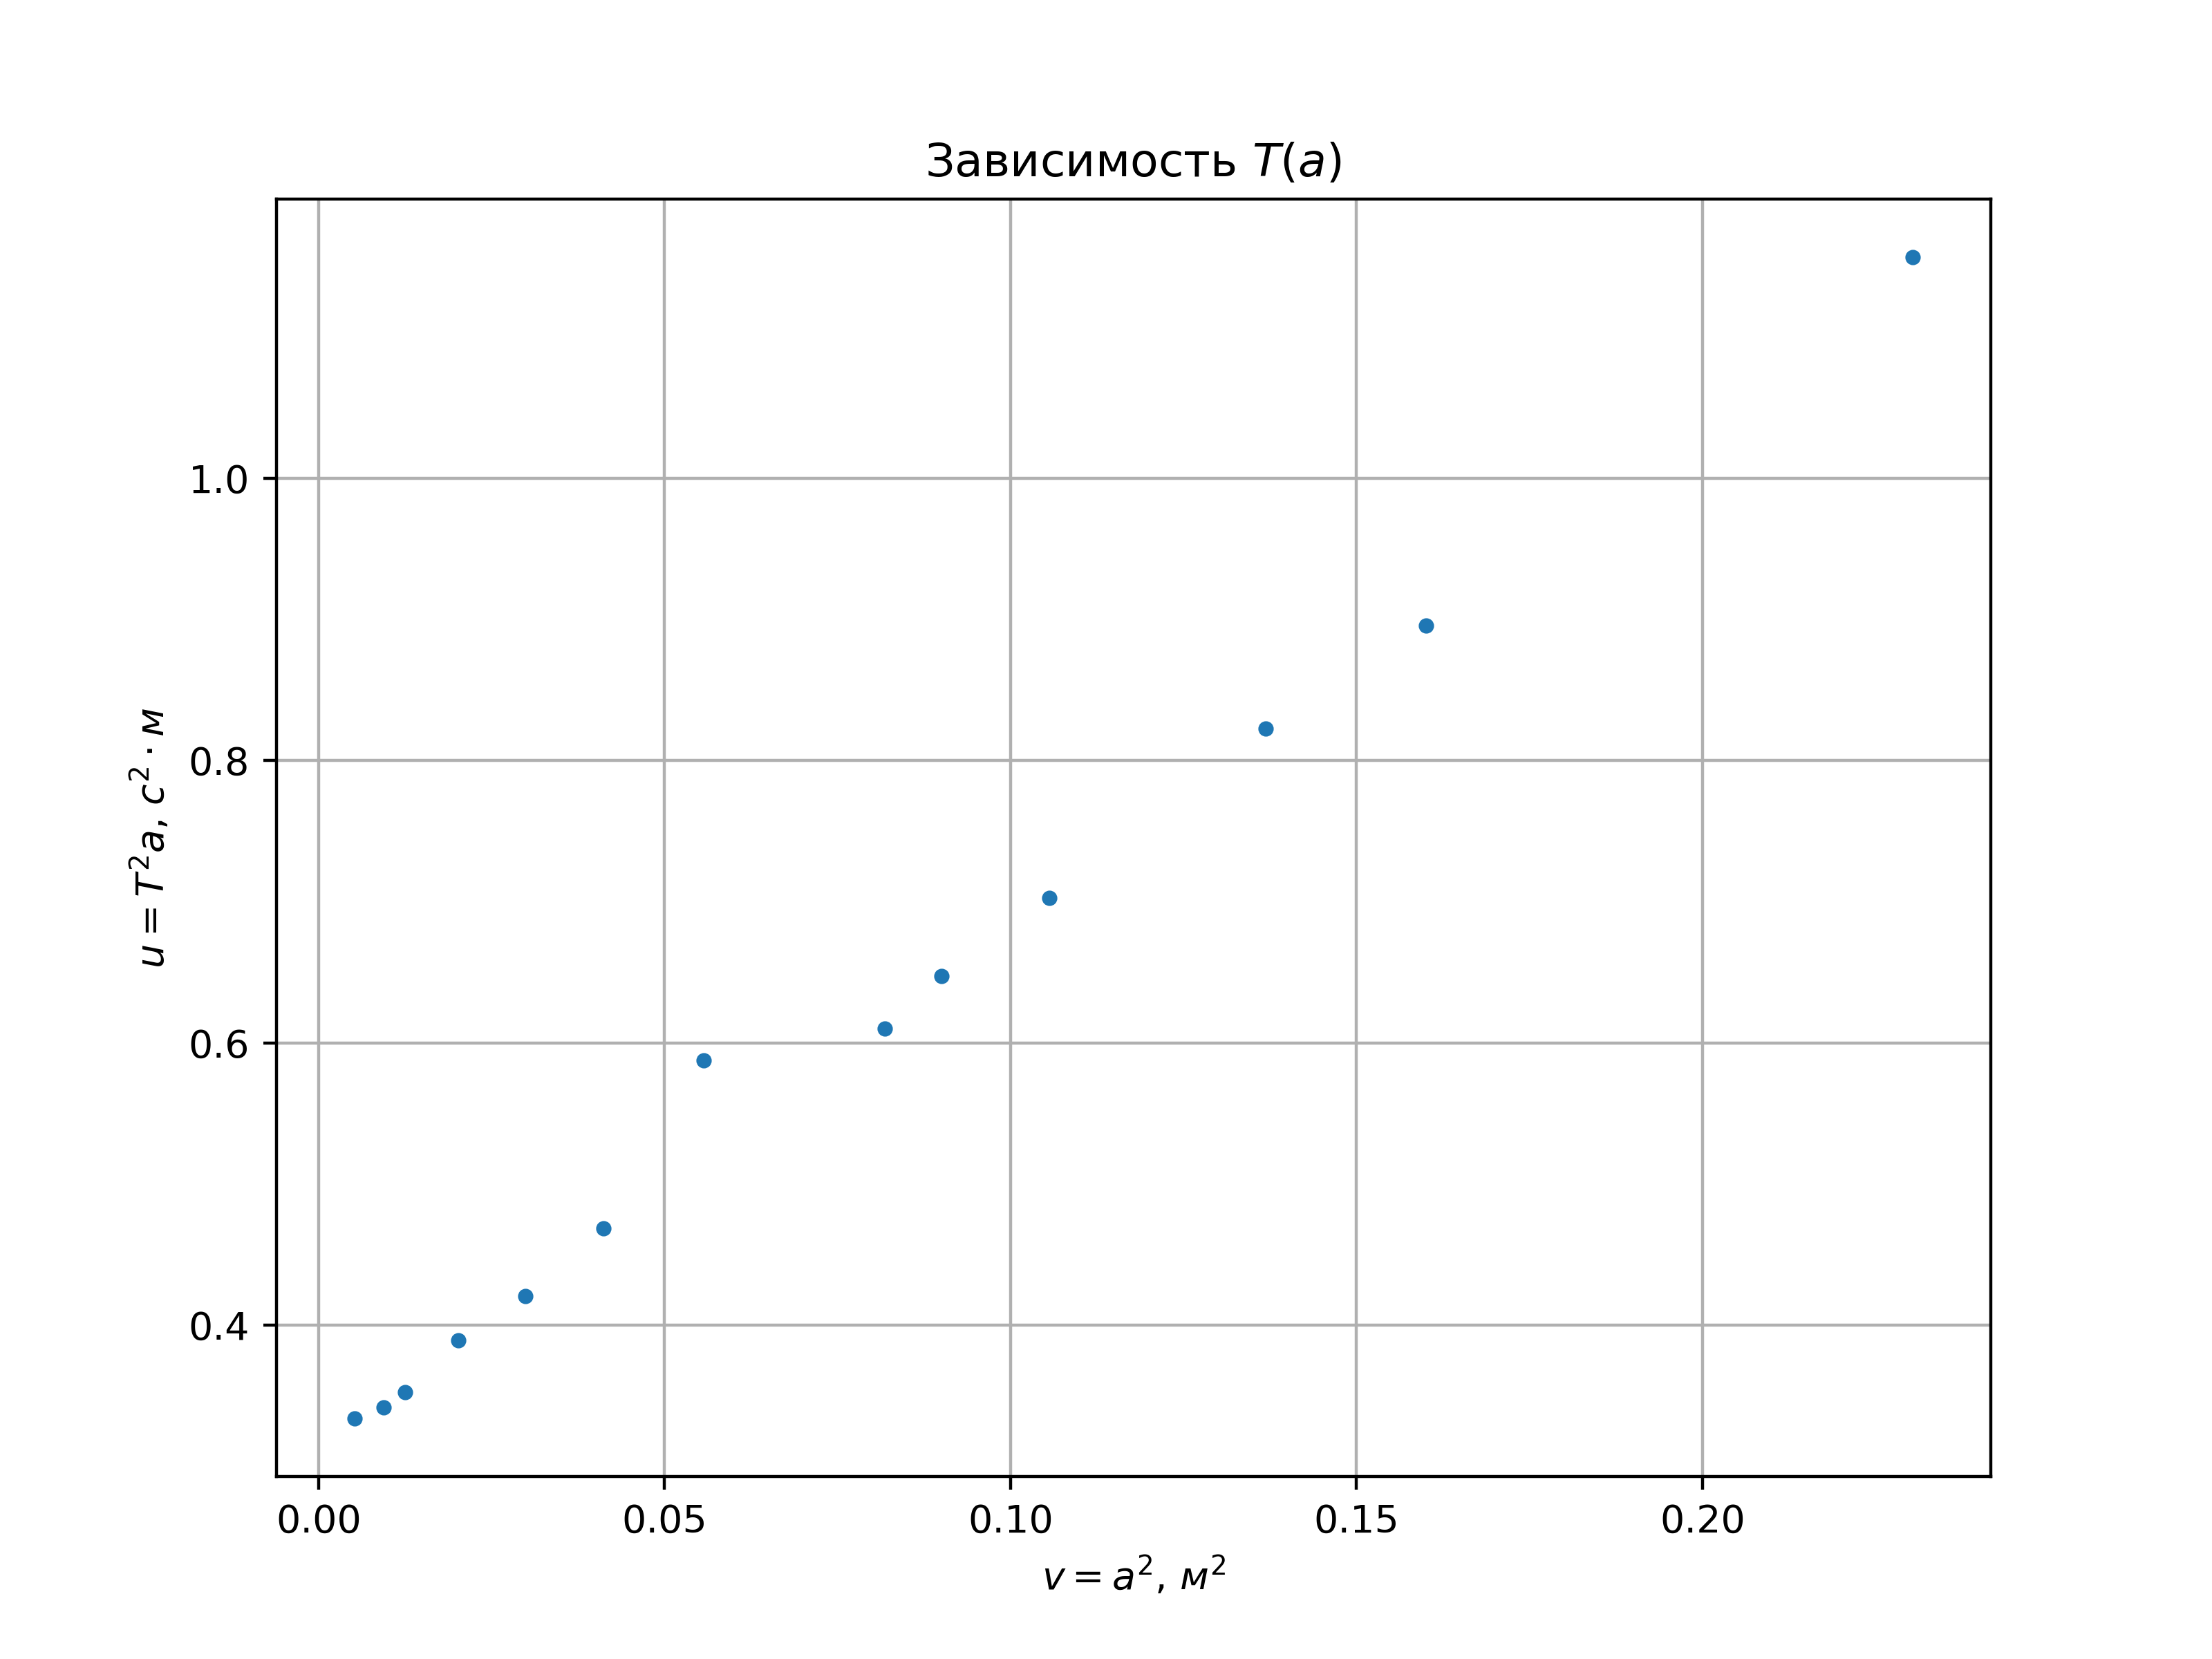
\includegraphics[width=0.8\linewidth]{img/a.png}
\end{figure}

\begin{figure}
    \centering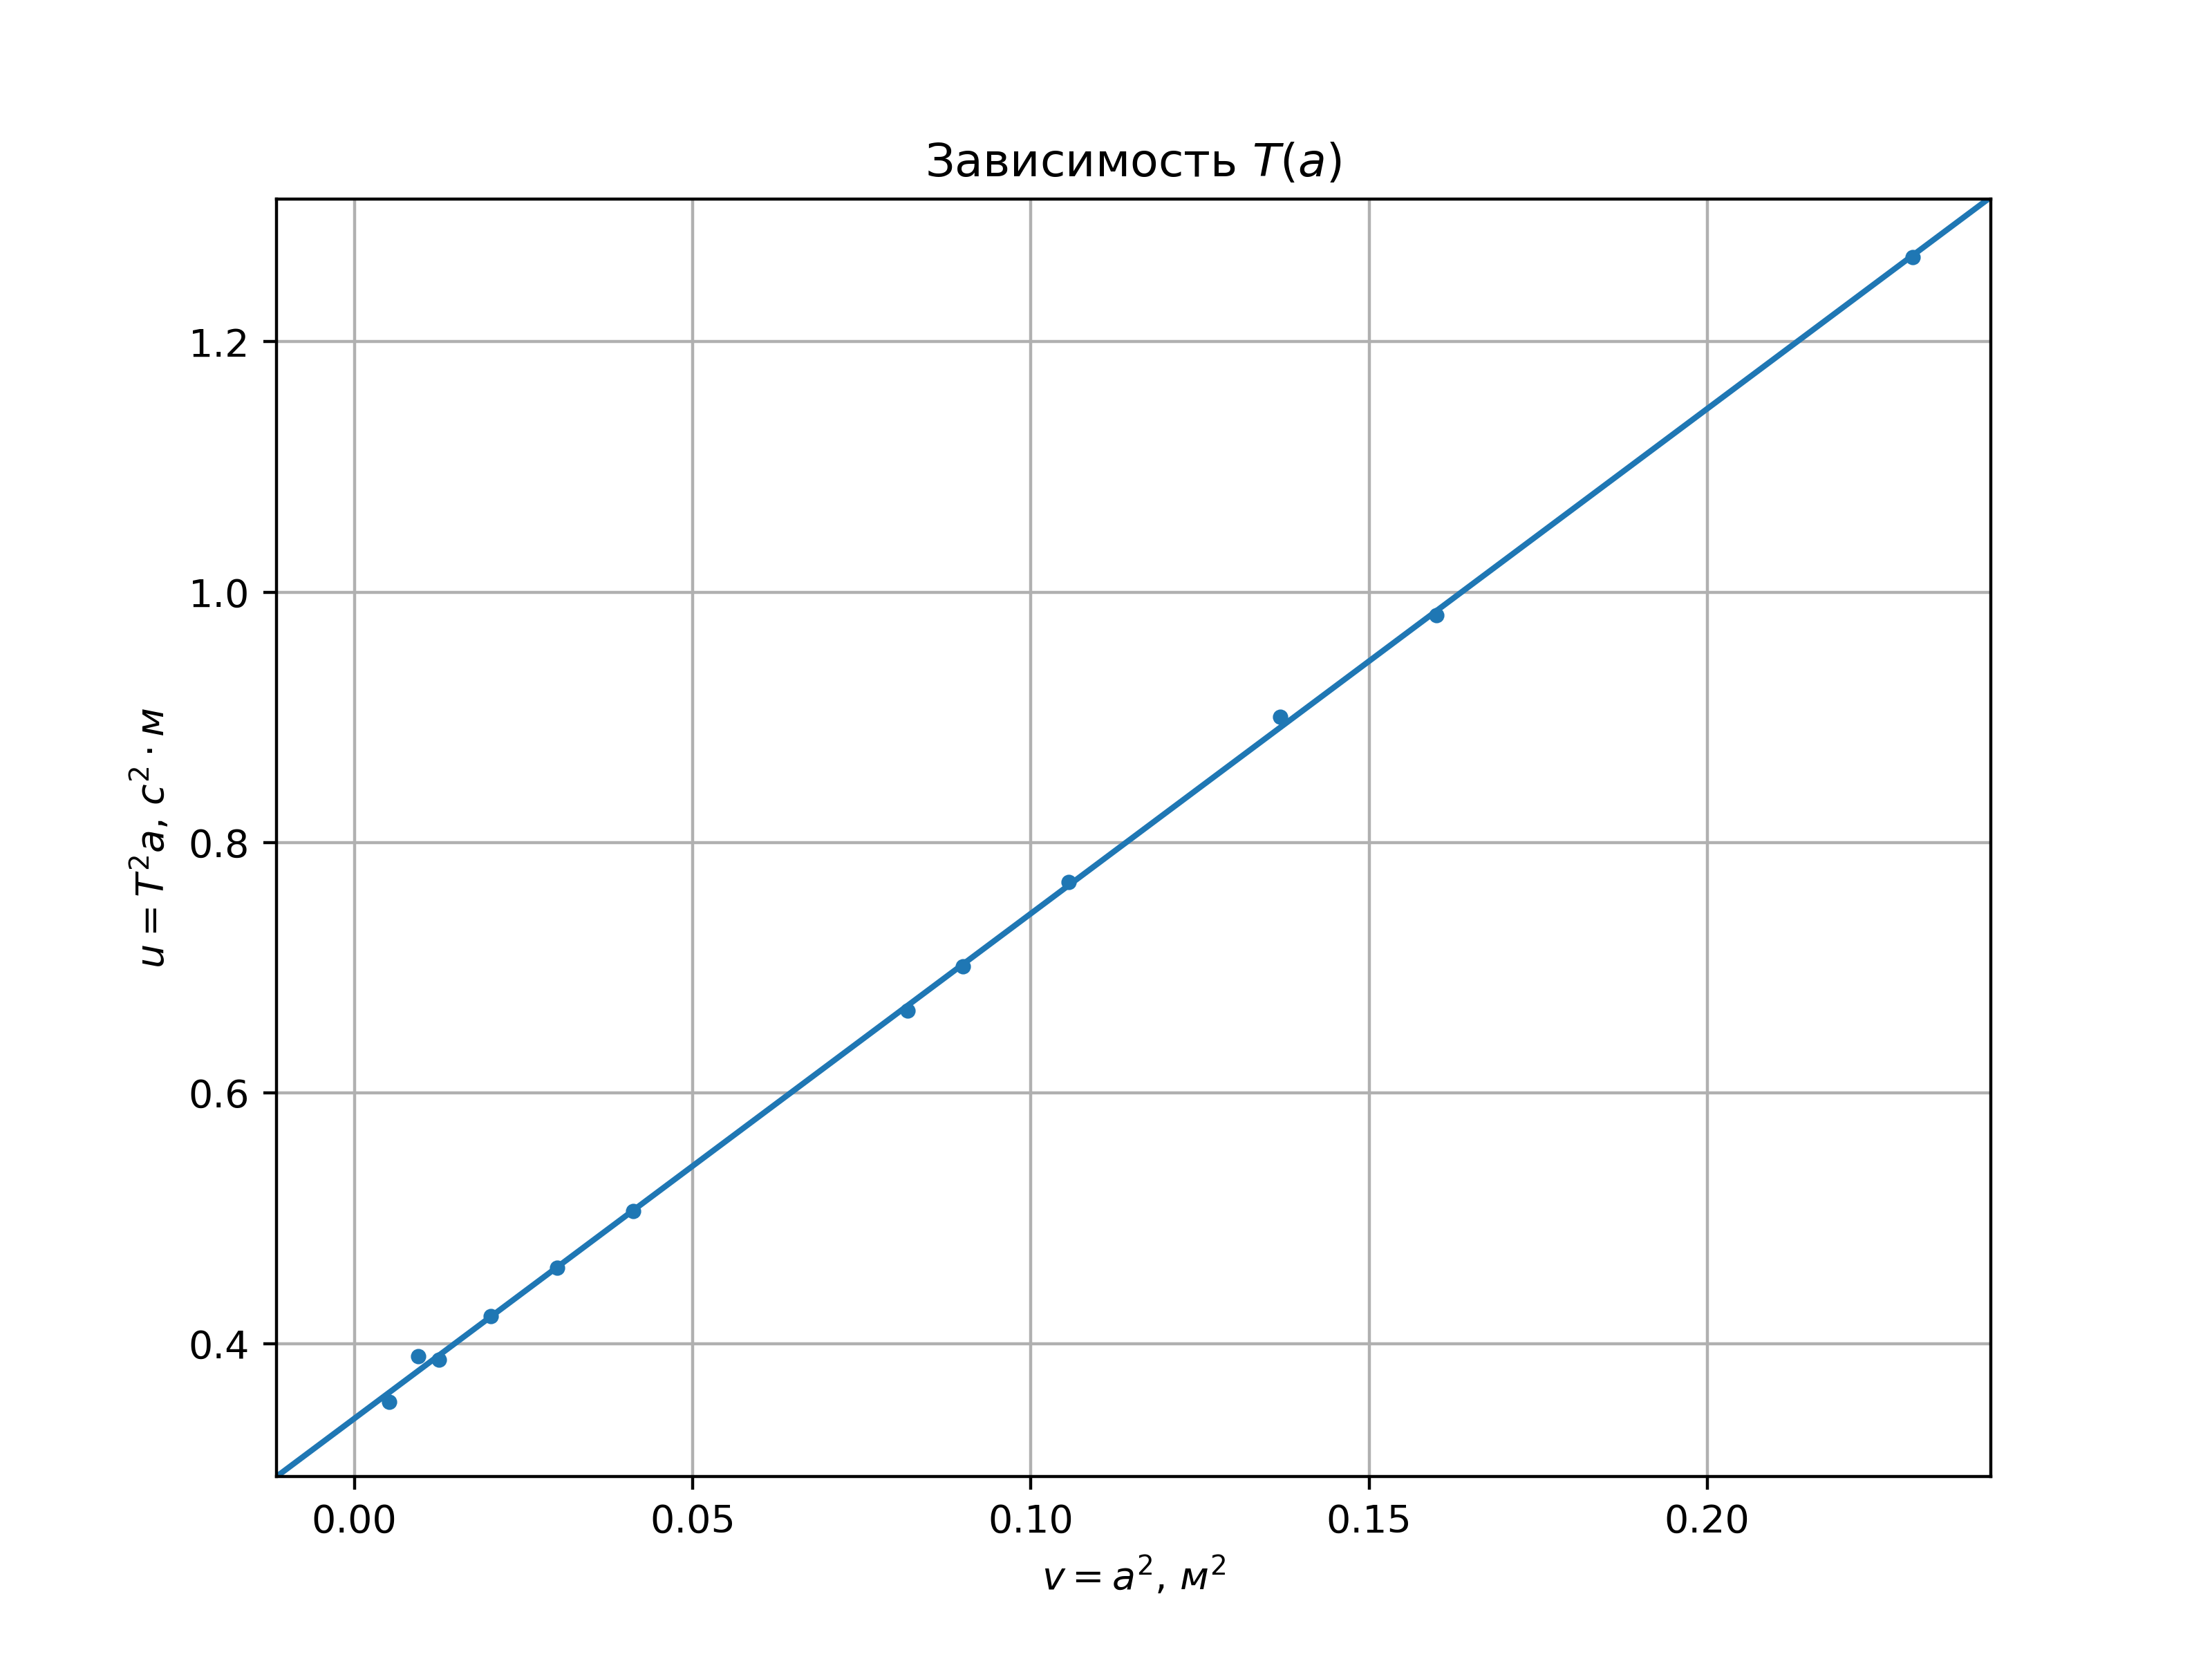
\includegraphics[width=0.8\linewidth]{img/b.png}
\end{figure}

Из графика $T_{min}\approx 1{,}53\,\text{с}$, $a_{min}\approx 0{,}29\,\text{м}$
Теоретическое значение $a_{min}=a/\sqrt{12}\approx 289\,\text{мм}$, что совпадает
с полученным значением.

Параметры прямой на графике (исключая выбросную точку) $k=4{,}03\pm 0{,}02\,\text{c}/\text{м}$, 
$b=0{,}3402\pm0{,}0014\,\text{м}\cdot\text{с}^2$.

\[g=\frac{4\pi^2}{k}\]
\[g=9{,}79\pm 0{,}06\,\text{м}/\text{с}^2\]

Погрешности измерений $a$ и $T$ очень малы ($\varepsilon_a\approx 0{,}002$
на большинстве точек, $\varepsilon_T < 0{,}001$), ими можно пренебречь по сравнению
со случайной погрешностью $\varepsilon_k\approx 0{,}005$.

Расчёт по графику предпочтительнее, т.к. позволяет исключить выбросные точки.

Амплитуда маятника уменьшилась в 2 раза за $t=330{,}02\,\text{с}$, совершив при этом
221 колебание. Тогда $\gamma=\ln 2/t\approx 2\cdot 10^{-3}\,\text{с}^{-1}$,
$\tau = 1/\gamma\approx 476\,\text{с}$, $Q=\pi\cdot n/\ln 2\approx 1000$.
